\chapter{Offline Planning Policies}

\section{Policy-Environment Matchups}

It may not be immediately obvious that a strategy for switching between altitudes is helpful. The problem formulation used here is such that policies that only ever command drones to fly at Low altitude can still be guaranteed to complete coverage for all legal environments. However, this policy is not optimal for all environments. To understand this, consider the following toy instance of the coverage problem:

\begin{figure}[H]
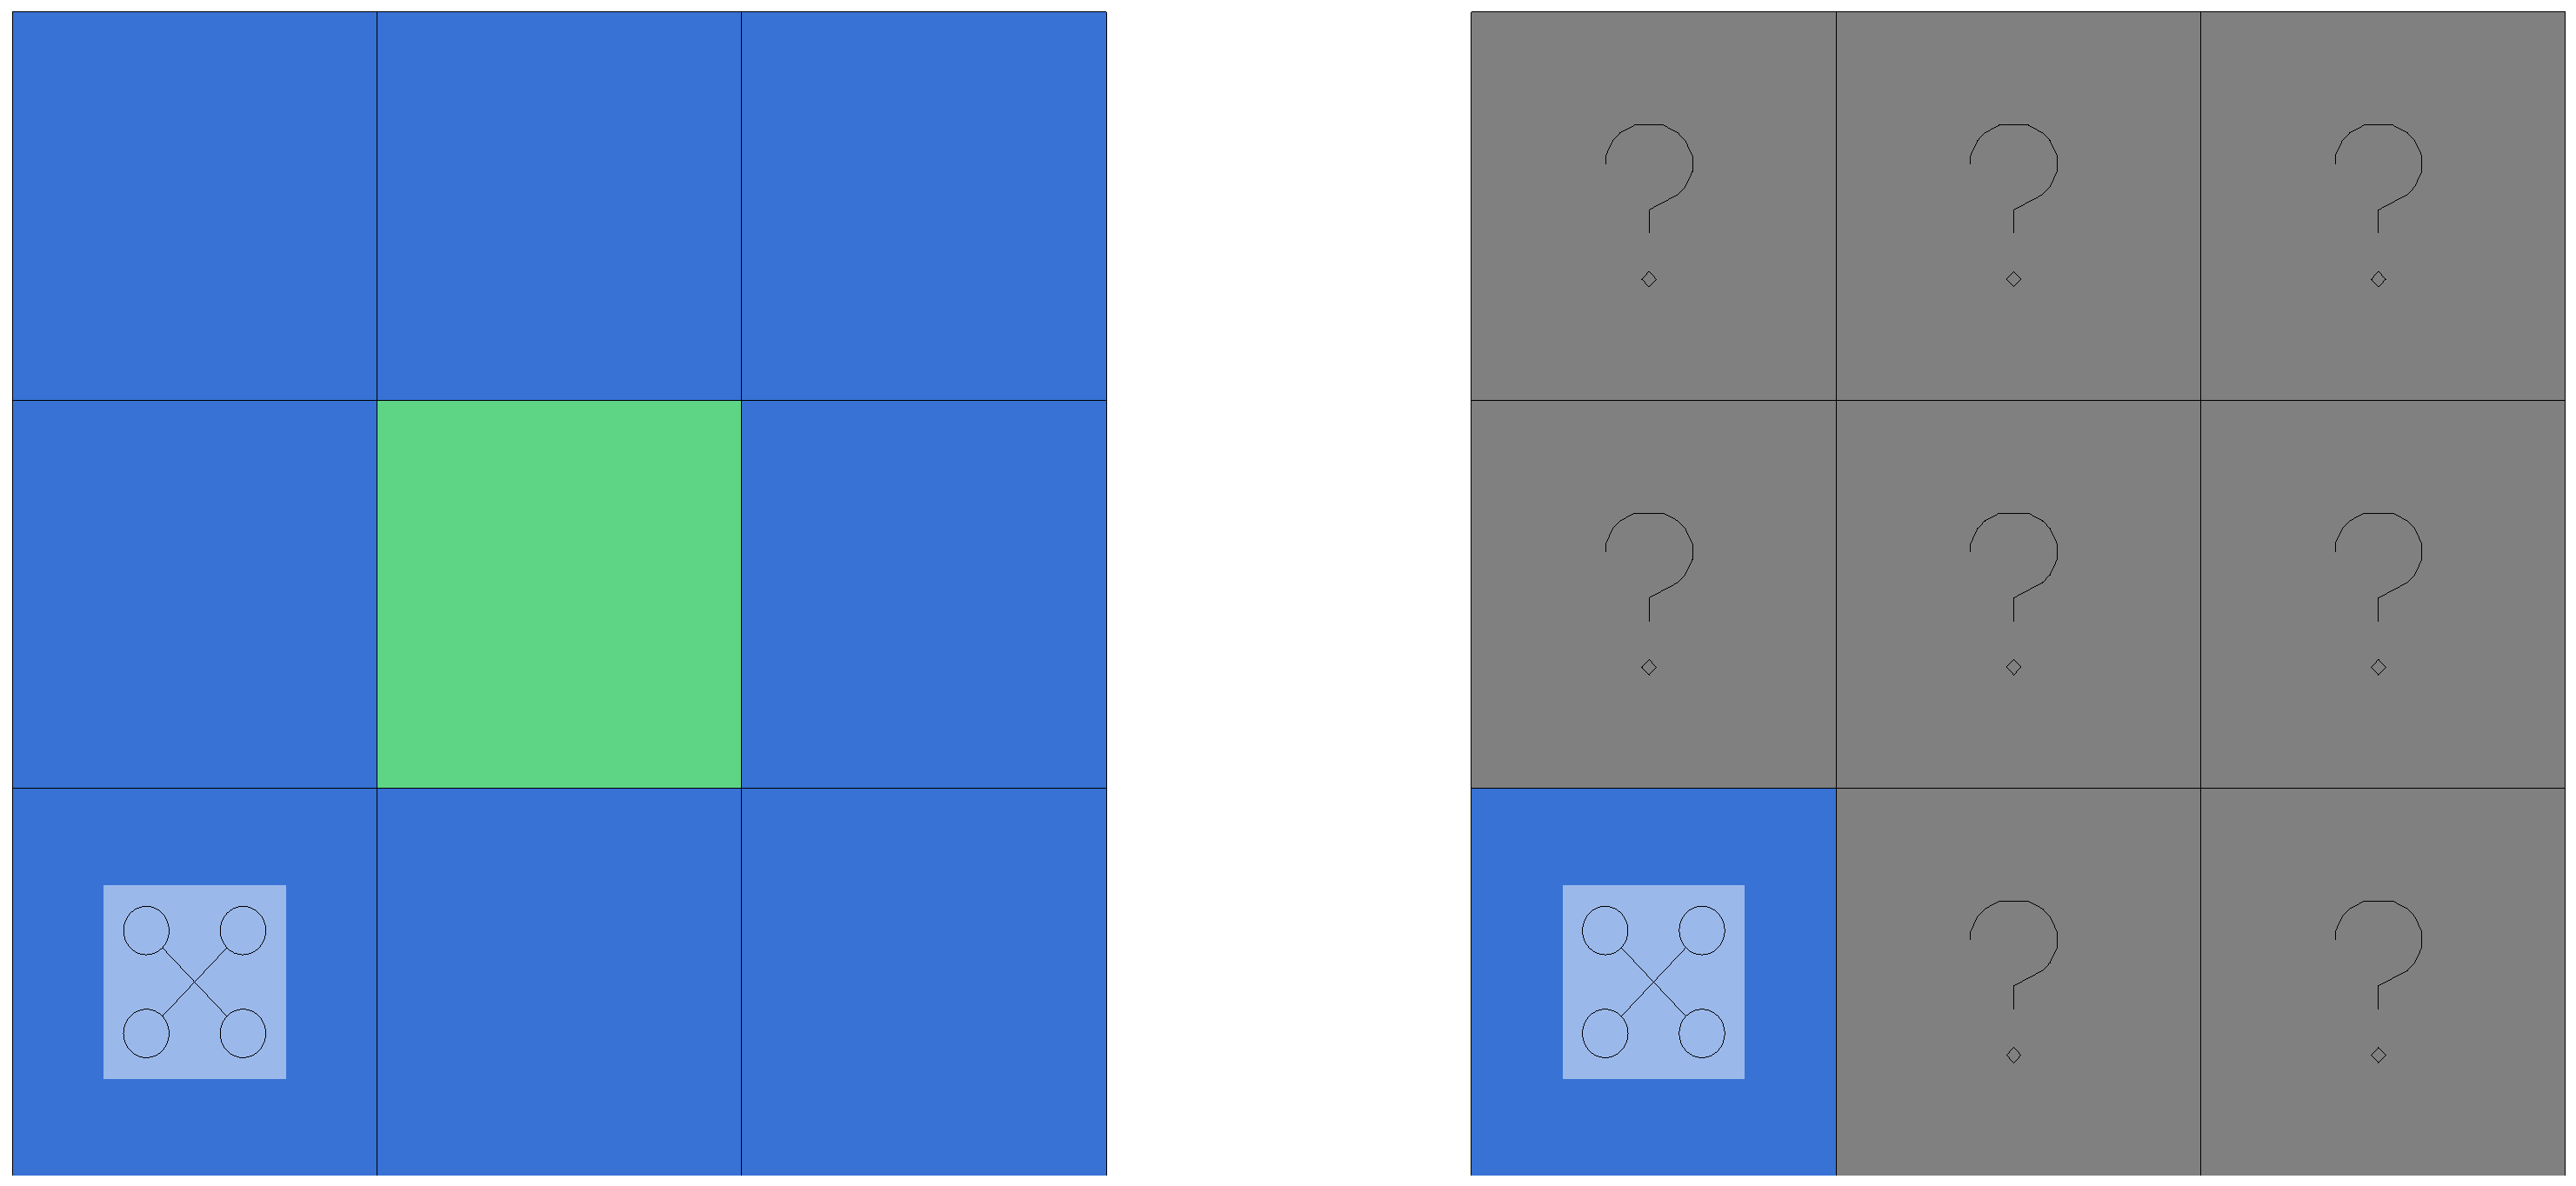
\includegraphics[width=\textwidth]{ex3Init}
\caption[Tiny Square Environment]{A drone sits at the lower left of a small environment. The right image indicates that it has only covered the patch directly below it so far.}
\label{fig:ex3-1-start}
\end{figure}

Assume that a single drone must cover this environment starting from a low altitude over position (0, 0). Because of this starting position, the drone starts with limited information about the environment (Figure \ref{fig:ex3-1-start} right). From here, there are a few viable strategies the drone could use to cover this environment.

\subsection{High Sweep First Policy}

One option that works well for this and other policies is to ascend to a high altitude, view every location in the environment with low scrutiny, then descend to cover any locations with a patch requiring a highly detailed view. In this case, because the drone starts from a low altitude, the first step in following such a policy is to ascend. This takes 10 steps and results in the following view of the environment:

\begin{figure}[H]
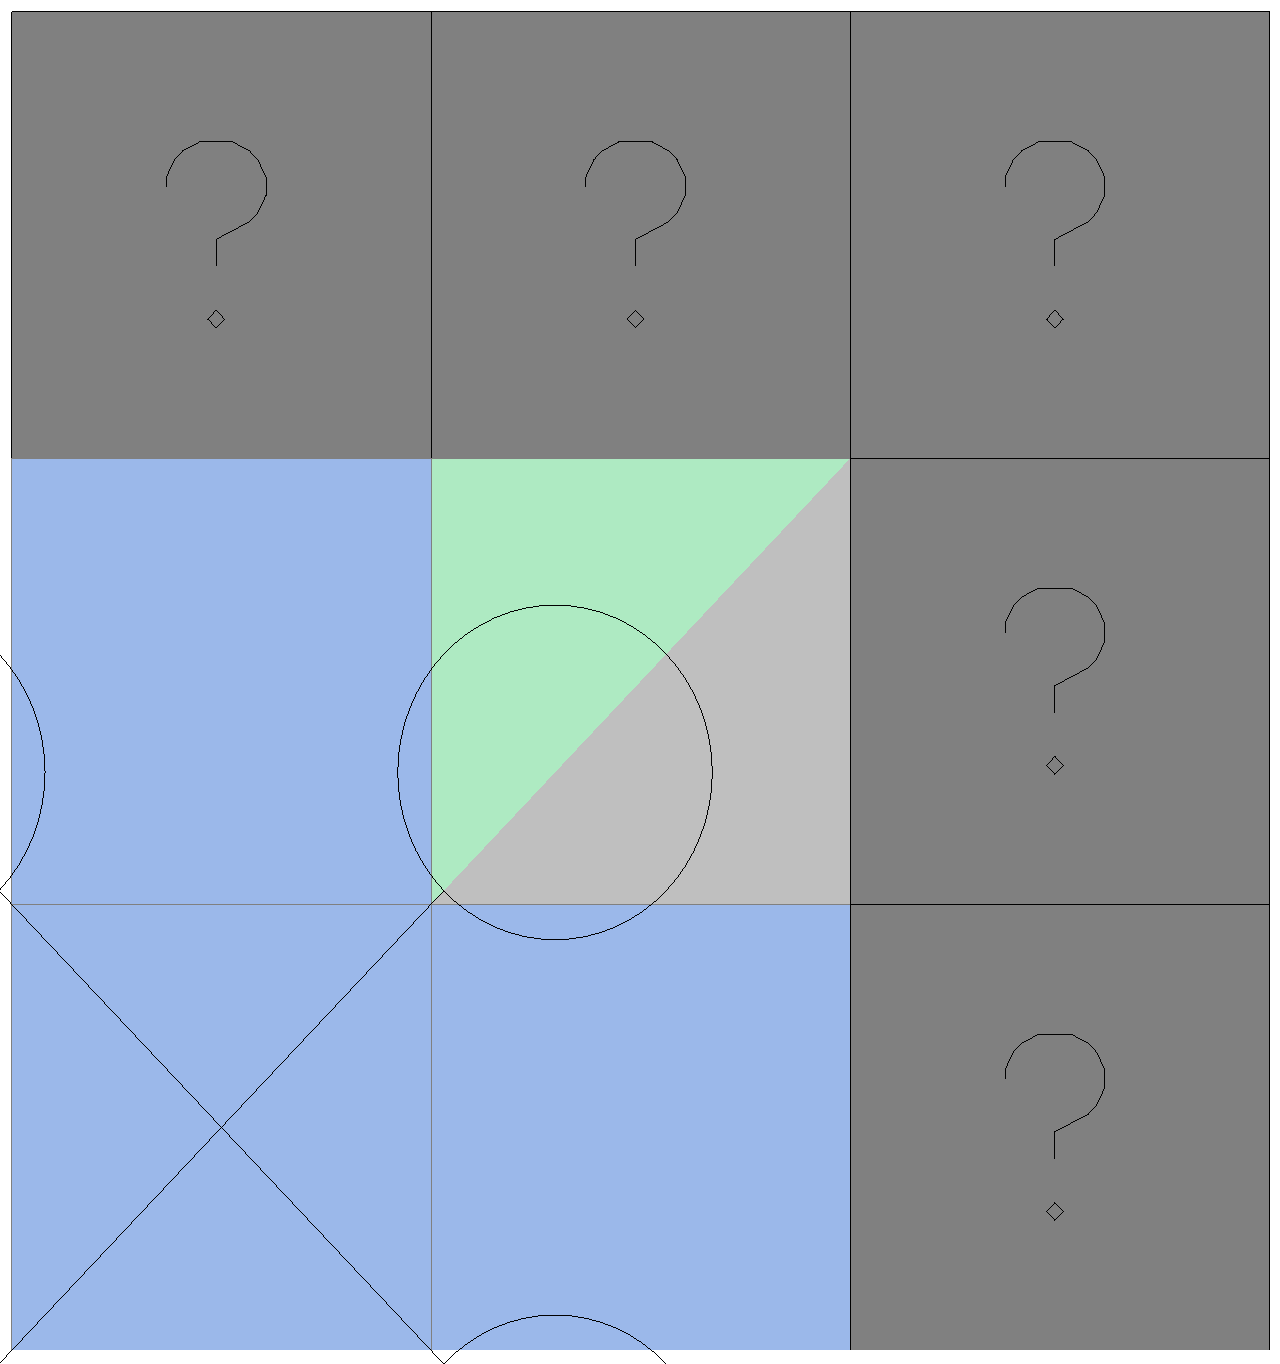
\includegraphics[width=0.5\textwidth]{3Middle1}
\caption[Partially Explored Environment]{The drone has ascended, giving it a view of the 3x3 grid of patches around its ground position.}
\end{figure}

Because this drone has ascended while flying over a corner position, there is not a full set of nine in bound patches for the drone to view at this moment. Instead, it can see the 2x2 group of patches that are within its field of view. The larger scale of the drone's high altitude field of view is indicated by enlarging the drone icon to cover an amount of the screen that corresponds to this much area on the drawn map.

From here, the High Sweep First Policy (HSFP) sends the drone to a position that takes full advantage of its large field of view, (1, 1). This is directly northeast of the drone's current location, so this position can be achieved by an intercardinal motion for 14 steps.

\begin{figure}[H]
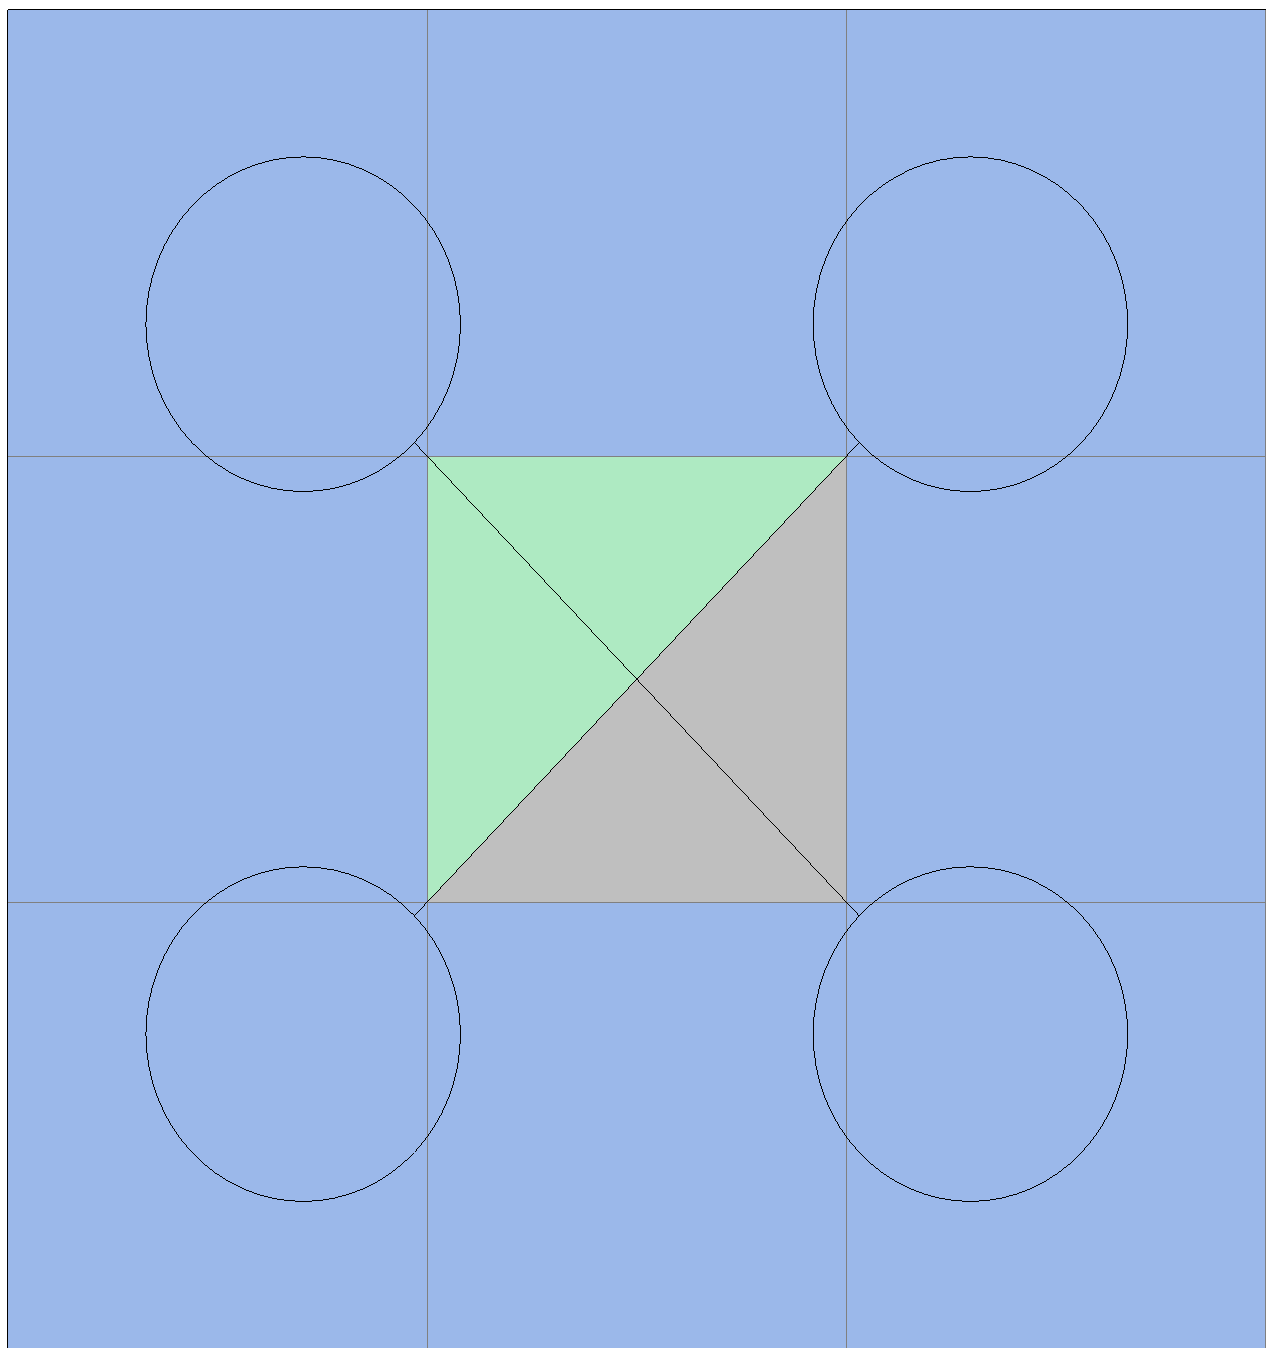
\includegraphics[width=0.5\textwidth]{3Middle2}
\caption[Complete information without complete coverage]{Complete information without complete coverage}
\end{figure}

From this vantage point, the drone is able to see a full 3x3 region of in bounds locations. This region happens to be the entire map. In addition, most of the locations in this environment have been drawn in blue, indicating that those locations can be covered with a low scrutiny view. Thus, all the drone needs to do is descend over the single patch requiring high scrutiny. Ten steps later, the task is complete:

\begin{figure}[H]
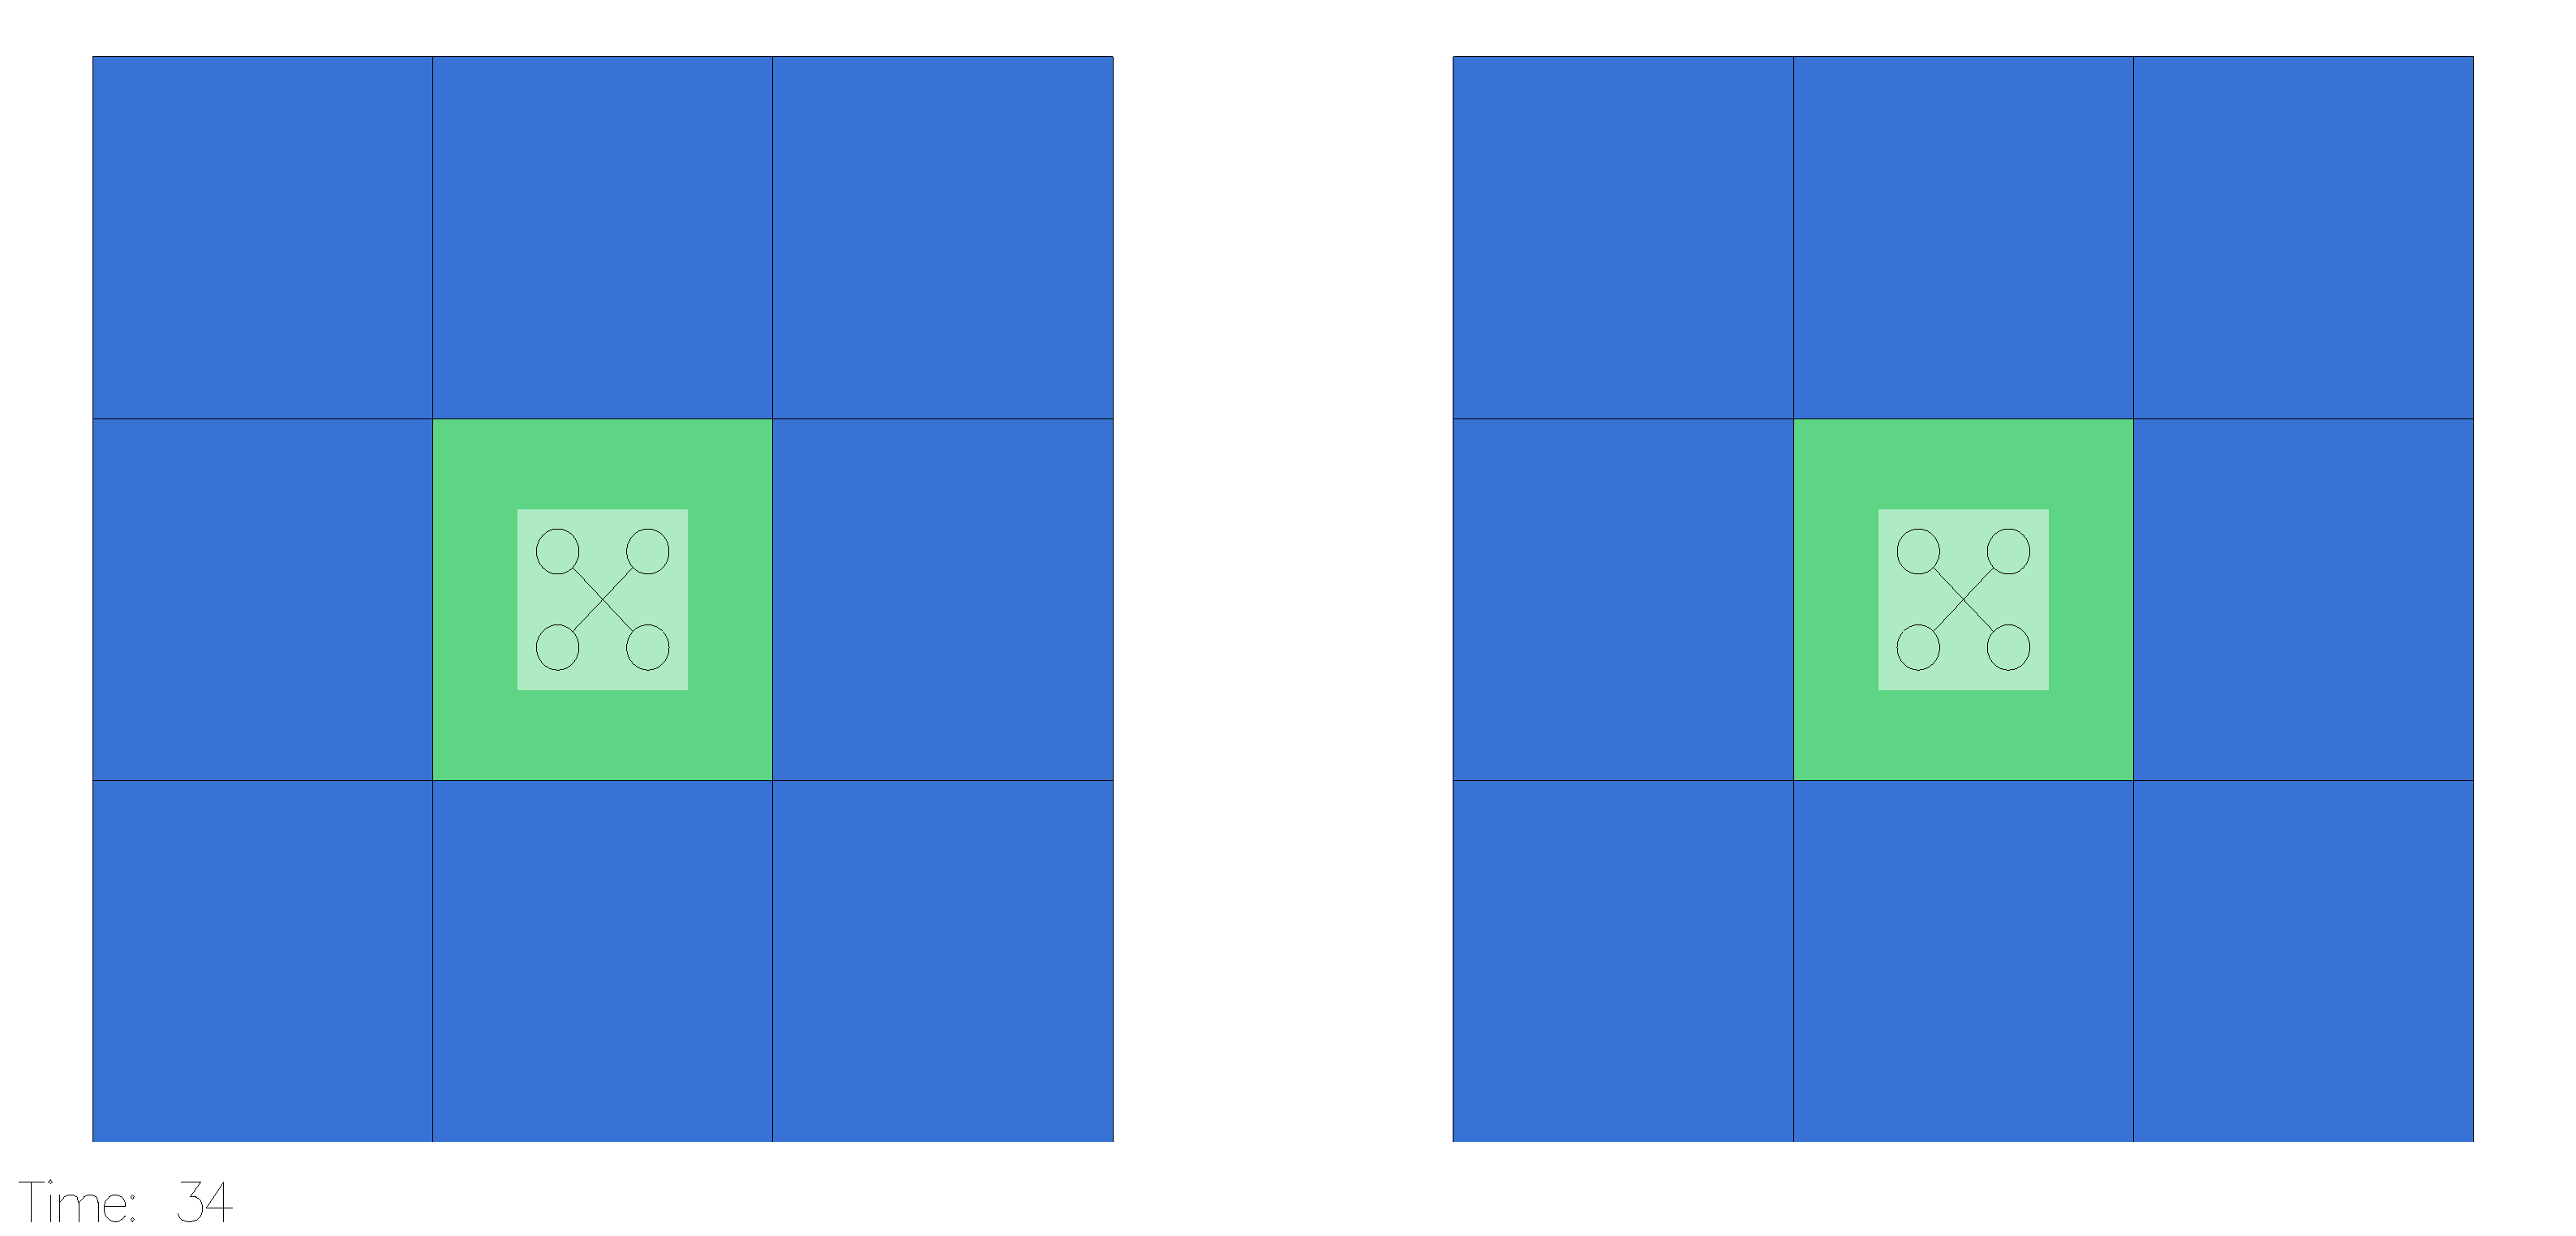
\includegraphics[width=\textwidth]{ex3-1-final}
\caption[Fully Covered Envrionment]{fully covered environment}
\label{fig:3-1-end}
\end{figure}

As shown in Figure \ref{fig:3-1-end}, this takes a total of 34 time steps. For this exact map, it's possible to achieve coverage in just 24 steps by moving northeast before ascending. However, given the decision to ascend at the first time step, this is the fastest possible task performance.

\subsection{Low Sweep Policy}

A second type of policy suitable for covering this environment is the low sweep policy (LSP). This policy snakes back and forth across the environment one column at a time. In order to achieve coverage of environments with more complex shapes, there are a few exceptions to that description which might not seem obvious when covering a simple environment such as the 3x3 in this example. In short, all locations in the environment will eventially be visited. Because any drone commanded by this policy will view all of its visited patches with high scrutiny, this policy is guaranteed to achieve complete coverage.

When exploring the same environment as before, this policy commands the following eight cardinal motions: [North, North, East, South, South, East, North, North]. These eight motions take a total of 80 time steps and result in a completely explored environment.

\subsection{Performance on an Alternate Environment}

The above example makes it seem like the "High Sweep First" approach may be the best choice for a policy to complete this task. However, this is also not the case for all environments. Consider the following environment, for which the relative performance of the same two policies from last time is flipped:

\begin{figure}[H]
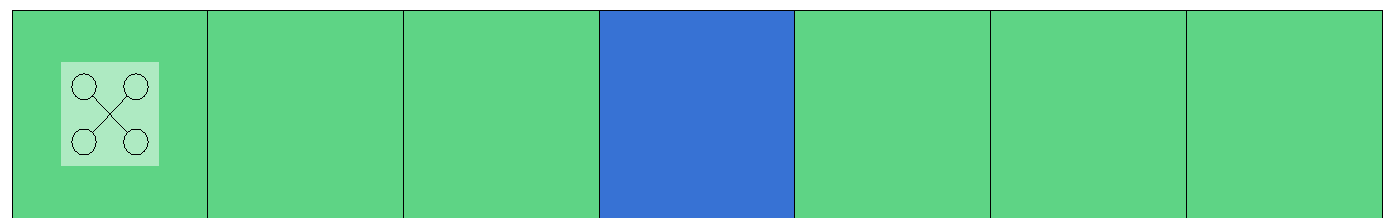
\includegraphics[width=\textwidth]{PrefLowEnv}
\caption[Long Thin Environment]{An environment with a different shape and dominant scrutiny requirement}
\label{fig:3-2-env}
\end{figure}

In this environment, HSFP does not do well at all. It ascends and flies most of the way across the environment, resulting in the following view:



%recreate the second environment from my wiki entry.

\subsection{Discussion}

Both of these examples used very small environments in order to limit the length of explanations required. On this small a scale, the size and shape of the environment's Footprint provides a strong hint about the appropriate altitude switching strategy to employ when exploring the environment. Because the environment's Footprint is available to an agent before any decision needs to be made, it may be possible to create a policy that optimizes its behavior around that factor somewhat. However, for large environments that mostly consist of wide open space, the importance of this contribution on a case by case basis is likely to be minimal. Setting aside considerations about Footprint shape, the different ratios of High vs Low scrutiny patches used in these examples provide the first hint that the a priori unknown content of each environment has implications for the best possible strategy. As an extremely simple proof that this is the case, consider the following tiny environments:

%1: HL
%1: L 

%2: HH
%2: H

In both cases, assume that there is a single drone that starts at the top left position at a Low altitude.

In the first case, the best possible solution is to immediately Ascend. This action, whose move cost is as low or lower than all other move costs available in this simulation, completes the coverage task. Thus, this is clearly the optimal policy to use for exploring this environment in particular. In the second case, all environment cells require High scrutiny, and so must each be visited from a Low altitude. This means that the drone must move to each of the following states before the coverage tasks is complete:

\begin{enumerate}
	\item Low over Position (1, 1)
	\item Low over Position (0, 0)
\end{enumerate}

In this case, one optimal policy would be to move East and then South-West. This policy causes the scenario to complete in 24 time steps. More importantly, any Policy that starts out with an Ascend would then need to Descend before any of the necessary observations to complete coverage can be performed. These two altitude switching moves require a total of 20 time steps to complete, making it clearly impossible to finish the task in less than the 24 time steps that another policy demonstrates. With that, it has been demonstrated that a policy's chance at optimally exploring either of these environments can be ruined at the \textit{very first} move performed. The set of moves which keep a possibility of optimality in the first environment, {Ascend}, and the set of moves that do the same in the second environment, {MoveCardinal East, MoveCardinal South}, are disjoint. All of this is true despite the fact that policies operating in these two environments must make a decision based on precisely the same initial information:

%:?L?

This proves that it is impossible to create a policy that makes optimal decisions without assuming some distribution of possible environments. The exact degree to which environment distributions will affect policy performance on larger environments is not addressed analytically in this work. However, as later sections will demonstrate, experimental results show that this difference is quite dramatic.

As discussed in the previous chapter, oprc\_env is capable of generating quite a large number of different environments. Even if the exact parameters used by a particular environment generator are known in advance, it is not easy to characterize the distribution of resulting environments in a way that is useful for fine-tuning the design of policies. In addition, it seems intuitively likely that the distribution of real world environments in which this coverage behavior would be useful is similarly complex. This chapter will discuss the development and experimental optimization of Policy instances that do a good job on a complex distribution of environments.